\documentclass[11pt]{exam}
\usepackage[margin=1in]{geometry}
\pagestyle{plain}
\usepackage{amsmath,amsfonts,amssymb,amsthm,enumerate}
\usepackage{multicol}
\usepackage[]{graphicx}
\usepackage{hyperref}
\usepackage{tikz}
\usepackage{pgfplots}
\usepackage{subfigure}
\usepackage[final]{pdfpages}

\newcommand{\plainanswer}[1]{\ifprintanswers #1 \fi}

\addtolength{\footskip}{2\baselineskip} % to lower the page numbers
\title{\vspace{-0.5in} Math 115 \\ Worksheet Section 1.8}
\date{}


% \theoremstyle{definition}
% \newtheorem{problem}{Problem}
\renewcommand{\questionlabel}{\textbf{Problem~\thequestion.}}
%\printanswers

\begin{document}
\maketitle
\vspace{-0.75in}
\begin{questions}
  \question (1.8 \#26) Find the following limit exactly, using algebra (not a table or graph):
	$\displaystyle\lim_{x \to 1} \frac{x^2-4x+3}{x^2+3x-4}$
        \begin{solution}
          \[
            \lim_{x \to 1}\frac{x^2-4x+3}{x^2+3x-4} = \lim_{x\to 1}
            \frac{(x-3)(x-1)}{(x+4)(x-1)} = \lim_{x\to
              1}\frac{x-3}{x+4} = \frac{1-3}{1+4} = -\frac{2}{5}
          \]
        \end{solution}
  \question First, find the left- and right-handed limits of the given function $f(x)$ at both $x=3$ and $x=5$.  Then find all values where $f(x)$ is not continuous.
	$$f(x) = \left\{ \begin{array}{ll} \displaystyle\frac{6-x}{x} & 0\leq x \leq 3
	\\ x^2-8x+17 & 3<x<5
	\\ 12-2x & 5\leq x \leq 6
	\end{array}
	\right.$$
        \begin{solution}
          \begin{itemize}
          \item \(\displaystyle\lim_{x\to 3^-} f(x) = \lim_{x \to 3^-}
            \frac{6-x}{x} = \frac{6-3}{3} = 1\)
          \item \(\displaystyle\lim_{x\to 3^+} f(x) = \lim_{x \to 3^+} x^2-8x+17 =
            3^2-8\cdot 3 + 17 = 9-24+17 = 2\)
          \item \(\displaystyle\lim_{x\to 5^-} f(x) = \lim_{x \to 5^-}
            x^2-8x+17 = 25-40+17 = 2\) 
          \item \(\displaystyle\lim_{x\to 5^+} f(x) = \lim_{x \to 5^+}
            12-2x = 12-10 = 2\)
          \end{itemize}
          Thus, \(f(x)\) is not continuous at \(x=3\).
        \end{solution}
        \vspace{1in}
  \question Find the following limits, or say they do not exist (DNE)
  and justify your answer.
  \begin{parts}
    \part $\displaystyle  \lim_{x\to \infty}
    \frac{9x^3-x+83}{x^4}=\plainanswer{0 \text{ since }x^4\text{
        dominates }9x^3-x+83}$
    \part $\displaystyle  \lim_{x\to \infty}
    \frac{x^4}{9x^3-x+83}=\plainanswer{\infty  \text{ (DNE) since }x^4\text{
        dominates }9x^3-x+83}$
    \part $\displaystyle  \lim_{x\to \infty}
    \frac{9x^3-x+83}{x^3}=\plainanswer{9\text{ since the }x^3\text{
        terms dominate the numerator and denominator}}$\plainanswer{\\
        This yields \(\frac{9x^3}{x^3}=9\)}
    \part $\displaystyle  \lim_{x\to \infty}
    \frac{2e^x+5}{3e^x+7}=$\plainanswer{\(\frac{2}{3}\) since the
      \(e^x\) terms dominate the numerator and denominator. \\ This
      yields \(\frac{2e^x}{3e^x} = \frac{2}{3}\)}
    \part $\displaystyle  \lim_{x\to \infty}
    \frac{2^{-x}+5}{3^{-x}+7}=$\plainanswer{\(\frac{5}{7}\) since the
      \(2^{-x}\) and \(3^{-x}\) tend to \(0\) as \(x \to \infty\).}
    \part$\displaystyle  \lim_{x\to \infty}
    \frac{2^{x}+5}{3^{x}+7}=$\plainanswer{\(0\) since the \(2^x\)
      dominates the numerator, the \(3^x\) dominates the denominator,
      and thus we get the same behavior as \(\frac{2^x}{3^x} = \left(
        \frac{2}{3} \right)^x\) as \(x\to\infty\), yielding \(0\). }
    \part$\displaystyle  \lim_{x\to -\infty}
    \frac{e^{-x}}{x}=$\plainanswer{\(\infty\) (DNE) since \(e^{-x}\)
      dominates \(x\) as \(x\to -\infty\).}
  \end{parts}
  \question On the board, draw the graph of a function $f$ that has
  all the following properties:
	\begin{itemize}
	\item $\displaystyle  \lim_{x\to 3} f(x)=5$
	\item $f(3)=0$
	\item $\displaystyle  \lim_{x\to 0+} f(x)=4$
	\item $\displaystyle  \lim_{x\to 0} f(x)$ DNE
	\item $\displaystyle  \lim_{x\to -\infty} f(x)= +\infty$
	\end{itemize}
        \pagebreak
  \question (1.8 \# 6--8) If $\displaystyle\lim_{x\to 2}f(x)=7$, $\displaystyle\lim_{x\to 2}g(x)=4$, and $\displaystyle\lim_{x\to 2} h(x) = \frac{1}{2}$, find 
  \begin{parts}
    \part $\displaystyle\lim_{x\to 2} (f(x) - 2h(x))\plainanswer{ =
      \lim_{x\to 2}f(x) - 2\lim_{x\to 2}h(x) = 7-2\cdot\frac{1}{2} = 6}$
    \part $\displaystyle\lim_{x\to 2} (g(x))^2\plainanswer{ = \left( \lim_{x \to 2}
    g(x)\right)^2 = 4^2 = 16}$
    \part $\displaystyle\lim_{x\to 2}
    \frac{f(x)}{g(x)h(x)}\plainanswer{= \frac{\lim_{x\to
          2}f(x)}{\lim_{x\to 2}g(x) \lim_{x \to 2}h(x)} = \frac{7}{4
        \cdot \frac{1}{2}}= \frac{7}{2}}$
  \end{parts}
\question (Fall 2017 Exam 1)
If $q(x) = \frac{2e^{kx}}{1+2^x}$, find all values of $k$ such that $\displaystyle\lim_{x \rightarrow \infty}q(x) = 0$. If there are none, write NONE. Show your work or reasoning to justify your answer.
\begin{solution}
  See part (d) on \href{https://dhsp.math.lsa.umich.edu/exams/115exam1/f17/s9.pdf}{https://dhsp.math.lsa.umich.edu/exams/115exam1/f17/s9.pdf}
\end{solution}
\vspace{0.5in}
\question (Winter 2018 Exam 1) \begin{enumerate}[(a)]
\item Let $p(x)$ be a polynomial satisfying all the following properties: 
\begin{enumerate}[(i)]
\item $p(x) = 0$ only at $x = -2, 0, 3$.
\item $\displaystyle\lim_{x \rightarrow - \infty} p(x) = - \infty$ and $\displaystyle\lim_{x \rightarrow \infty} p(x) = - \infty$.
\end{enumerate}
Find one possible formula for $p(x)$. There may be more than one correct answer.

\item Let $h(x)$ be a rational function satisfying all the following properties:
\begin{enumerate}[(i)]
\item$\displaystyle\lim_{x \rightarrow 2} h(x) = 0$ and $h$ is not defined at $x=2$.
\item $\displaystyle\lim_{x \rightarrow \infty} h(x) = 0$.
\end{enumerate}
\end{enumerate}
\begin{solution}
  See parts (b)--(c) on \href{https://dhsp.math.lsa.umich.edu/exams/115exam1/w18/s6.pdf}{https://dhsp.math.lsa.umich.edu/exams/115exam1/w18/s6.pdf}
\end{solution}
\question (Winter 2017 Exam 1) Find all real numbers $B$ and positive integers $k$ such that the rational function
$$H(x)= \frac{9+x^k}{16-Bx^3}$$
satisfies the following two conditions:
\begin{itemize}
\item $H(x)$ has a vertical asymptote at $x=2$.
\item $\displaystyle\lim_{x \rightarrow \infty} H(x)$ exists.
\end{itemize}
\begin{solution}
  See \href{https://dhsp.math.lsa.umich.edu/exams/115exam1/w17/s10.pdf}{https://dhsp.math.lsa.umich.edu/exams/115exam1/w17/s10.pdf}
\end{solution}
\question (Winter 2016 Exam 1)
Consider the function \(f(x)\) defined by
$$f(x) = \left\lbrace \begin{array}{ll} \! \! xe^{Ax} + B & \textrm{if } x<3 \\ \!\! C(x-3)^2 & \textrm{if } 3 \leqslant x \leqslant 5 \\ \!\! \frac{130}{x} & \textrm{if } x > 5
\end{array}\right.$$
Suppose $f(x)$ satisfies all of the following:
\begin{itemize}
\item $f(x)$ is continuous at $x=3$.
\item $\displaystyle\lim_{x \rightarrow 5^+} f(x) = 2 + \displaystyle\lim_{x \rightarrow 5^-} f(x)$.
\item $\displaystyle\lim_{x \rightarrow -\infty} f(x) = -4$.
\end{itemize}
Find the values of $A$, $B$ and $C$. You must give exact answers.
\begin{solution}
 See \href{https://dhsp.math.lsa.umich.edu/exams/115exam1/w16/s9.pdf}{https://dhsp.math.lsa.umich.edu/exams/115exam1/w16/s9.pdf}
\end{solution}
\pagebreak
\question (Winter 2018 Exam 1) Consider the functions $f(x)$ and $g(x)$ given by the formula and graph below.

$$f(x) = \left\lbrace \begin{array}{ll} 2x^3-2x^2 & \textrm{for } x \leqslant 1 \\x^3 + 1 & \textrm{for } x > 1 \end{array} \right.$$

  \begin{figure}[h]
    \centering
    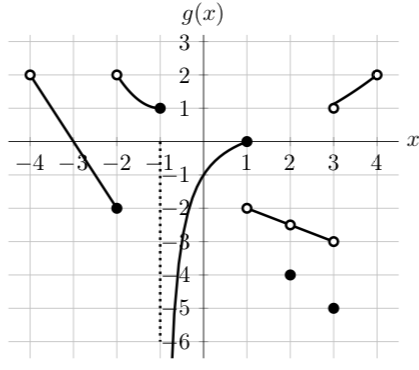
\includegraphics[scale=0.5]{discontinuities}
  \end{figure}

\begin{enumerate}[(a)]
\item Circle the correct answer(s) in each of the following questions.
\begin{enumerate}[(i)]
\item At which of the following values of $x$ is the function $g(x)$ not continuous?
$$\begin{array}{ccccccccccccc}
x = -3 &&& x = -1 &&& x = 0 &&& x = 2 &&& x = 3.5
\end{array}$$
\item At which of the following values of $x$ is the function $f(x) + g(x)$ continuous?
$$\begin{array}{ccccccccccccc}
x = -2 &&& x = -1 &&& x = 0 &&& x = 1 &&& x = 2
\end{array}$$

\end{enumerate}
Note that $g(x)$ is linear on the intervals $(-4,-2)$, $(1,2)$ and $(2, 3)$. All your answers below should be exact. If any of the quantities do not exist, write DNE.

\item Find $\displaystyle\lim_{x \rightarrow 2} (2f(x)+g(x))$.

\item Find $\displaystyle\lim_{x \rightarrow \infty} \frac{f(2x)}{x^3}$.

  
\item Find $\displaystyle\lim_{x \rightarrow \infty} g(x^2e^{-x} + 3)$.

\item For which values of \(p\) does $\displaystyle\lim_{x \rightarrow p^+} g(x)= 1$?

\item Find $\displaystyle\lim_{x \rightarrow -1^-} f(-x)$.
\end{enumerate}
\begin{solution}
 See \href{https://dhsp.math.lsa.umich.edu/exams/115exam1/w18/s8.pdf}{https://dhsp.math.lsa.umich.edu/exams/115exam1/w18/s8.pdf}
\end{solution}
\pagebreak
\question (Fall 2017 Exam 1) The graph of a functions $Q(x)$ with domain $[-5,5]$ is shown below.

\begin{figure}[h]
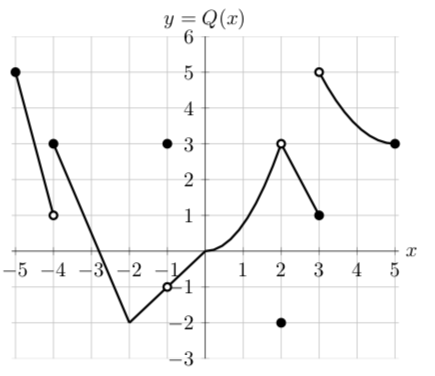
\includegraphics[scale=0.5]{discontinuities2}
\end{figure}
\begin{enumerate}[(a)]
\item Find the numerical value of the following mathematical expressions. If the answer cannot be determined with the information given, write “NI”. If any of the quantities does not exist, write “DNE”.
\begin{enumerate}[(i)]
\item Find $\displaystyle\lim_{x \rightarrow -1} Q(x)$.

\item Find $\displaystyle\lim_{w \rightarrow 2} Q(Q(w))$.

\item Find $\displaystyle\lim_{x \rightarrow \infty} Q \left( \frac{1}{x} + 3 \right)$.

\item Find $\displaystyle\lim_{x \rightarrow \frac{1}{3}} x Q \left( 3x-5 \right)$.
\end{enumerate}
\item For which values of $-5<p<5$ is $\displaystyle\lim_{x \rightarrow p^-} Q \left( x \right) \neq Q(p)$?
\end{enumerate}
\begin{solution}
  See \href{https://dhsp.math.lsa.umich.edu/exams/115exam1/f17/s4.pdf}{https://dhsp.math.lsa.umich.edu/exams/115exam1/f17/s4.pdf}
\end{solution}
\end{questions}

\end{document}
%%% Local Variables:
%%% mode: latex
%%% TeX-master: t
%%% End:
